% VLDB WORKSHOP template version of 2024-05-15 enhances the ACM template, version 1.7.0:
% https://www.acm.org/publications/proceedings-template
% The ACM Latex guide provides further information about the ACM template.

\documentclass[sigconf, nonacm]{acmart}

\newcommand\vldbyear{2026}
\newcommand\vldbworkshop{15th International Workshop on Quality in Databases (QDB’26)}
\newcommand\vldbauthors{\authors}
\newcommand\vldbtitle{\shorttitle}
\newcommand\vldbavailabilityurl{}
\newcommand\vldbpagestyle{plain}

\begin{document}

\title[Credibility Measurement in Social Media]{Measuring Credibility in Social Media Platforms through Data Quality and Provenance}

\author{Sebasti\'an Garc\'ia Parra}
\affiliation{%
  \institution{Facultad de Ingenier\'ia, Universidad de la Rep\'ublica}
  \city{Montevideo}
  \country{Uruguay}
}
\email{dgparra@fing.edu.uy}

\author{Adriana Marotta}
\affiliation{%
  \institution{Facultad de Ingenier\'ia, Universidad de la Rep\'ublica}
  \city{Montevideo}
  \country{Uruguay}
}
\email{amarotta@fing.edu.uy}

\begin{abstract}
Social media platforms have become primary sources of information for health,
politics, crises, and everyday decisions. Yet users often consume and propagate
content without explicit indicators about its credibility, especially when
content is copied, revised, or shared across platforms. We present a
data-quality model for measuring the credibility of social media clips. The model
organizes credibility around two main dimensions: trustworthiness, computed from
reputation, verifiability, and expertise, and provenance, which captures the
origin and evolution of a clip. We introduce Trustworthiness Path Stability, a
quality metric that evaluates whether trustworthiness remains stable along a
provenance path. We also describe a modular processing flow that normalizes clips
from heterogeneous platforms, generates domain-specific features, computes
quality metrics, and reconstructs provenance using explicit interactions and
textual equivalence. A proof of concept on posts about statins and cholesterol,
validated with a medical-domain expert, matches the expert judgment for nine of
eleven selected clips and illustrates how provenance can change the final
credibility assessment.
\end{abstract}

\maketitle

%%% do not modify the following VLDB block %%
%%% VLDB block start %%%
\pagestyle{\vldbpagestyle}
\begingroup\small\noindent\raggedright\textbf{VLDB Workshop Reference Format:}\\
\vldbauthors. \vldbtitle. VLDB \vldbyear\ Workshop: \vldbworkshop.\\
\endgroup
\begingroup
\renewcommand\thefootnote{}\footnote{\noindent
This work is licensed under the Creative Commons BY-NC-ND 4.0 International License. Visit \url{https://creativecommons.org/licenses/by-nc-nd/4.0/} to view a copy of this license. For any use beyond those covered by this license, obtain permission by emailing \href{mailto:info@vldb.org}{info@vldb.org}. Copyright is held by the owner/author(s). Publication rights licensed to the VLDB Endowment. \\
\raggedright Proceedings of the VLDB Endowment.
ISSN 2150-8097. \\
}\addtocounter{footnote}{-1}\endgroup
%%% VLDB block end %%%

%%% do not modify the following VLDB block %%
%%% VLDB block start %%%
\ifdefempty{\vldbavailabilityurl}{}{
\vspace{.3cm}
\begingroup\small\noindent\raggedright\textbf{VLDB Workshop Artifact Availability:}\\
The source code, data, and/or other artifacts have been made available at \url{\vldbavailabilityurl}.
\endgroup
}
%%% VLDB block end %%%

\section{Introduction}

Social media content is increasingly used as evidence for decisions that have
online and offline consequences. Users may decide whether to share a post, trust
a source, accept medical advice, or reject a treatment based on information whose
quality is uncertain. This risk is amplified by the way social media platforms
encourage rapid sharing and by the lack of standards for preserving quality
metadata when content crosses platform boundaries.

Existing platform mechanisms, such as verified accounts or community annotations,
provide useful signals but do not provide a general data-quality view of
credibility. Moreover, users commonly participate in several platforms, and
content may be copied manually, quoted, paraphrased, or reposted without carrying
the metadata available in the original platform. Thus, the same information item
may appear in multiple versions, with different authors, evidence, audience
signals, and trust contexts.

This issue is not only a matter of misinformation detection. Many existing
approaches classify a post, a topic, or a source as credible or not credible, but
they often hide the reasons behind the score. For data-quality assessment, this is
unsatisfactory: a consumer, a journalist, or a domain expert needs to know whether
a low score comes from missing evidence, weak source expertise, poor reputation,
or an unstable propagation path. The goal of this work is therefore to make
credibility measurable, decomposable, and auditable.

This paper focuses on credibility measurement in social media from a data-quality
perspective. Its main contribution is a provenance-aware model for clips, where a
clip denotes a social media information unit such as a post, tweet, comment,
video caption, or platform-specific publication. The model is platform agnostic
and domain adaptable: a data-quality expert defines the dimensions and metrics,
while a domain expert adjusts weights and thresholds for a concrete use case.

The contributions are threefold. First, we define a quality model for credibility
that combines trustworthiness and provenance. Second, we introduce
Trustworthiness Path Stability, a metric that captures how trust changes as
content is propagated and transformed. Third, we present a modular processing
flow and a medical-domain proof of concept on social media content about statins
and cholesterol.

\section{Background, Related Work, and Requirements}

Credibility has long been treated as a perceived quality rather than an inherent
property of an object~\cite{FoggTseng1999}. In data-quality terms, credibility is
related to trustworthiness, reputation, and provenance~\cite{BatiniScannapieco2016}.
For social media, this relation is especially important because credibility is
evaluated under uncertainty: users often see only a fragment of the original
context, and the perceived authority of an author may be misleading.

Prior work on information credibility in Twitter/X has shown that message
features, user features, topic features, and propagation features can help
estimate credibility~\cite{Castillo2011}. Other work studies social media data
quality directly and adapts traditional data-quality dimensions to streams of
tweets~\cite{Arolfo2020}. Recent work on adult readers' credibility evaluation of
social media posts reports that author biographies, perceived domain expertise,
and consistency with prior beliefs influence how evidence is judged~\cite{Kuutila2024}.

Provenance provides a complementary view. Data provenance captures origin,
derivation, and transformations, and has been recognized as a central mechanism
for assessing trust in data products~\cite{Simmhan2005}. PROV-SAID extends W3C
PROV to represent information diffusion in social media~\cite{Taxidou2015}. It
models messages, agents, influence, and interactions, but its original formulation
is centered on information diffusion within social platforms and does not directly
model cross-platform sharing or quality metrics attached to the provenance path.

\begin{table*}[t]
  \caption{Positioning of the proposed model with respect to related work.}
  \label{tab:related-gap}
  \small
  \begin{tabular}{@{}p{.20\textwidth}p{.36\textwidth}p{.37\textwidth}@{}}
    \toprule
    Line of work & Main focus & Remaining gap\\
    \midrule
    Web and social credibility & Multidimensional credibility cues and user perception & Limited operationalization as auditable data-quality metrics\\
    Twitter/X credibility models & Classification using message, user, topic, and propagation features & Platform-specific models with limited provenance-aware data-quality interpretation\\
    Social media data quality & Quality dimensions for social media streams & Credibility is not modeled as a provenance-aware quality cluster\\
    Social media provenance & Origin, diffusion, and interaction modeling & Quality metrics are not integrated into provenance paths\\
    \bottomrule
  \end{tabular}
\end{table*}

Table~\ref{tab:related-gap} summarizes the main related lines of work and their
remaining gaps. The gap addressed in this paper is not the absence of credibility
classifiers or
provenance models. Rather, the gap is the lack of a data-quality model that makes
credibility decomposable, provenance-aware, and reusable across social media
platforms and domains. Existing credibility approaches often estimate a label or
score from platform-specific features, while provenance approaches model
diffusion and derivation without attaching domain-specific quality metrics to the
path. Our proposal bridges these lines by treating credibility as a quality
cluster and by using provenance not only as traceability metadata but also as an
input to the credibility score.

These observations lead to four design requirements. The model must be platform
agnostic, because credibility signals vary across X, Facebook, TikTok, Reddit,
WhatsApp, and other platforms. It must be provenance aware, because the same
content may become more or less credible as it is copied, revised, or shared. It
must support domain-specific quality metrics, because credibility in medicine,
politics, and emergency response depends on different evidence. Finally, it must
be modular, so new feature generators, metrics, and provenance search strategies
can be incorporated without redesigning the whole flow.

A further requirement is interpretability. The proposed model is intended to be
used by different roles: end users who consume credibility indicators, data
quality experts who configure metrics, and domain experts who validate weights,
thresholds, and examples. For that reason, the model avoids treating credibility
as a black-box label and instead exposes the quality dimensions that contribute to
the final result.

\section{Credibility Quality Model}

We model \emph{Credibility} as a quality cluster composed of two main dimensions:
\emph{Trustworthiness} and \emph{Provenance}. Trustworthiness estimates the
expected reliability of the clip in its domain. Provenance captures the origin,
derivation, and propagation path of the clip.

\begin{figure*}[t]
  \centering
  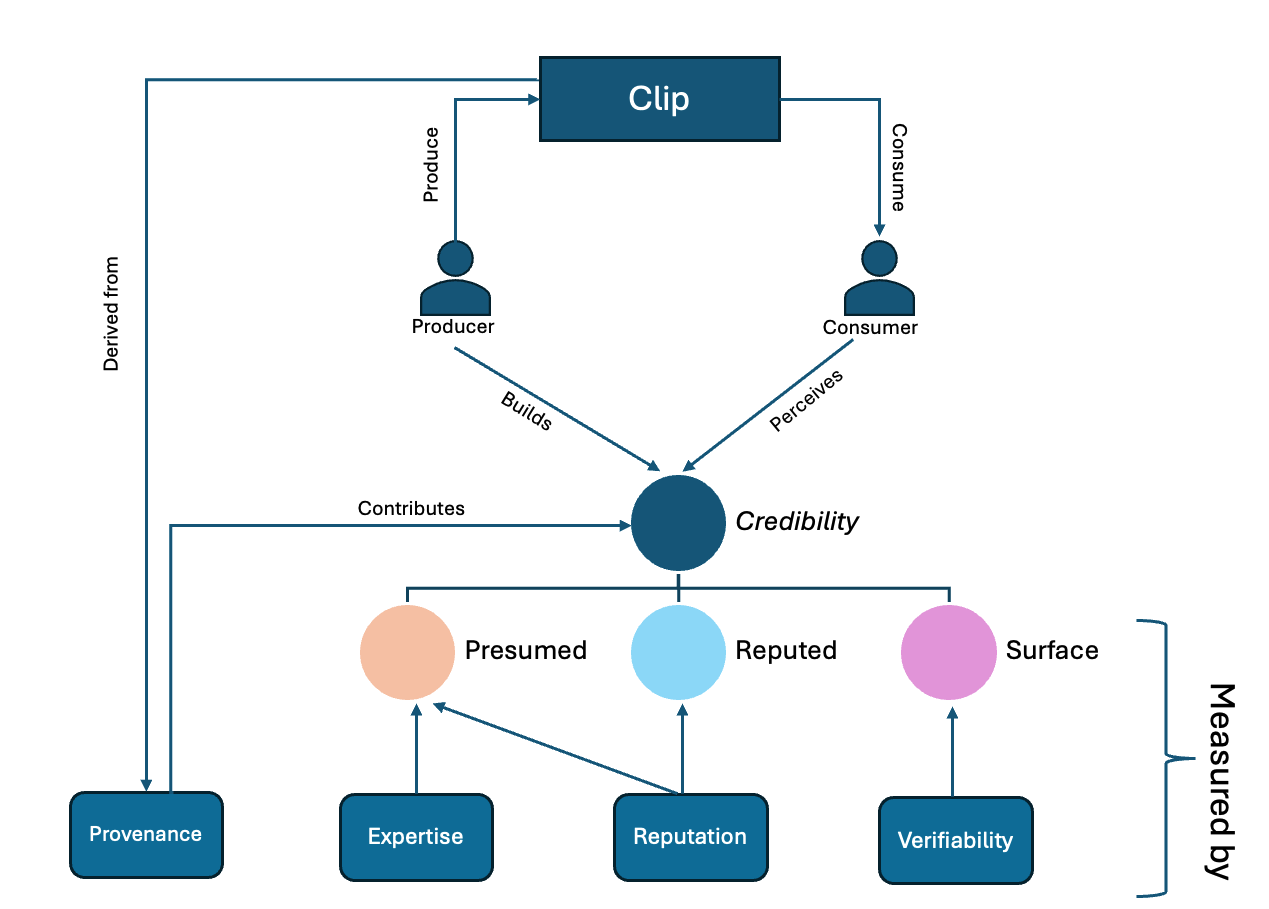
\includegraphics[width=.82\textwidth,height=.42\textheight,keepaspectratio]{figures/credibility-dq-composition-en}
  \caption{Conceptual composition of credibility and its associated quality dimensions~\cite{GarciaParra2024Thesis}.}
  \Description{Diagram showing a producer, a consumer, a clip, perceived credibility, and the quality factors expertise, reputation, verifiability, and provenance.}
  \label{fig:credibility-composition}
\end{figure*}

\begin{figure*}[t]
  \centering
  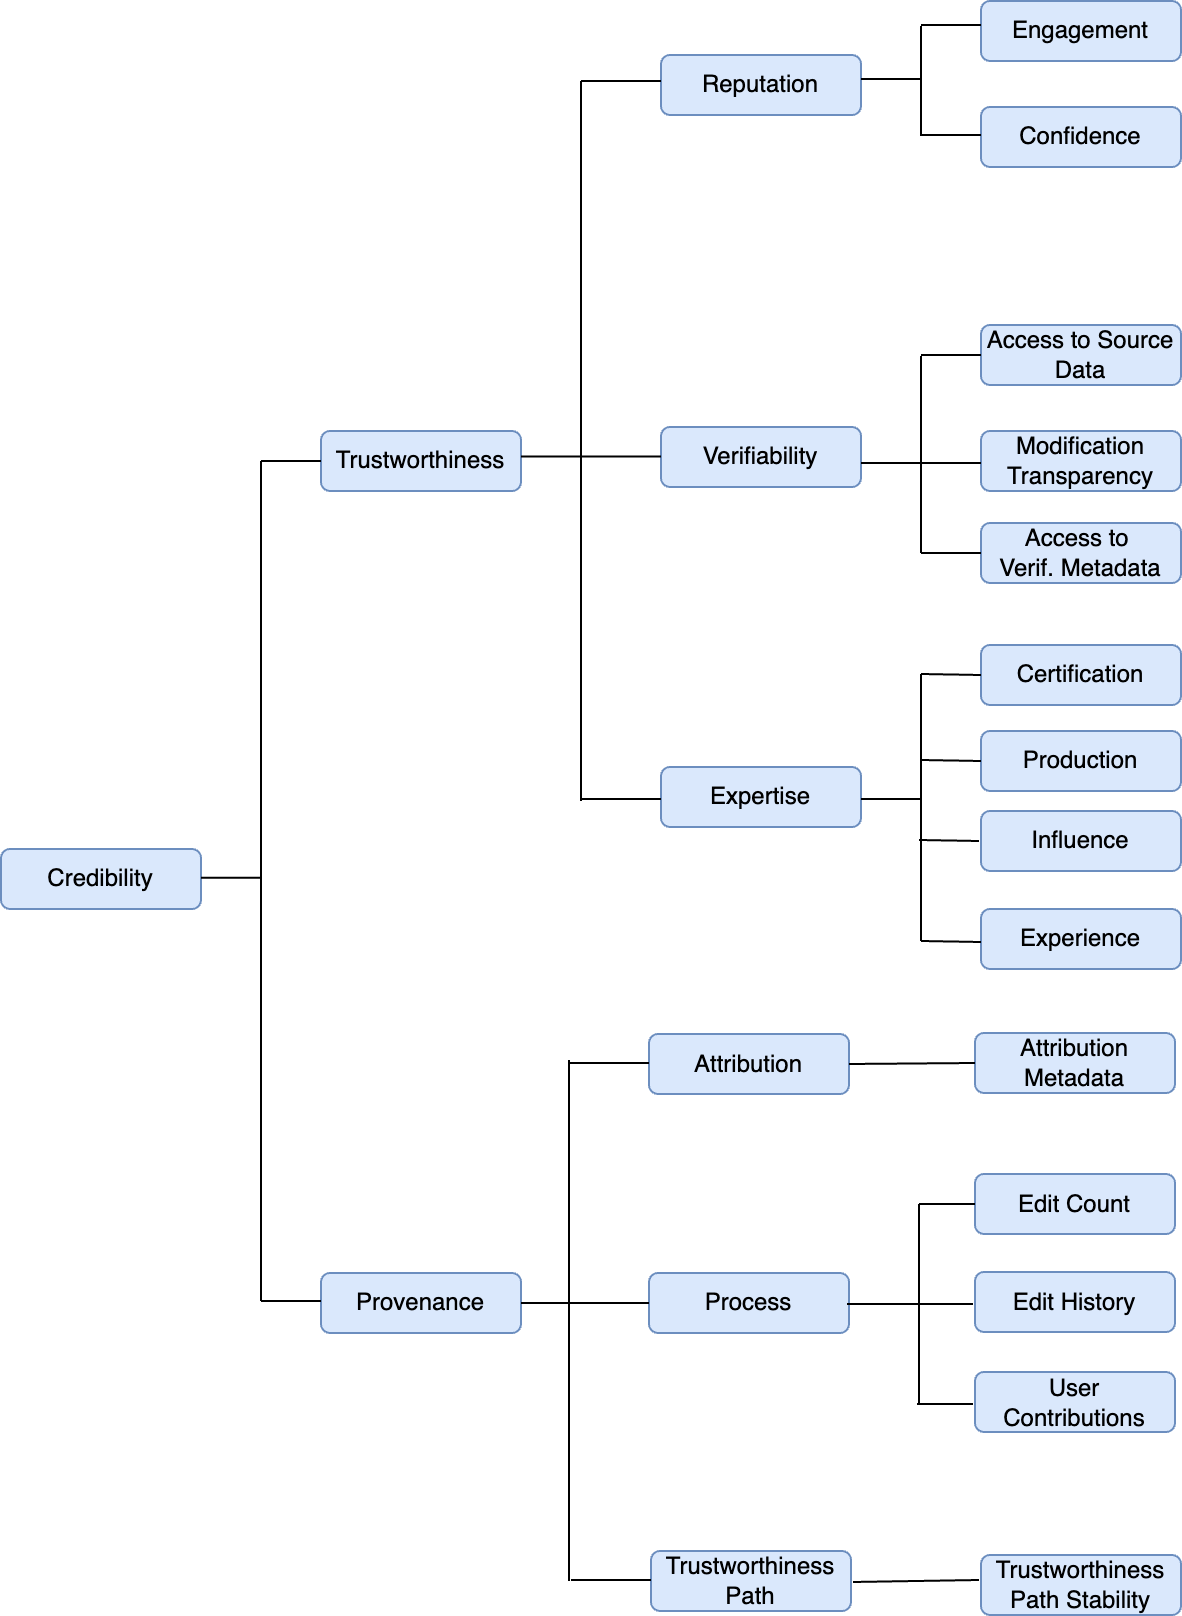
\includegraphics[width=.82\textwidth,height=.70\textheight,keepaspectratio]{figures/credibility-cluster-white}
  \caption{Credibility quality cluster~\cite{GarciaParra2024Thesis}.}
  \Description{Hierarchy of credibility, trustworthiness, provenance, and their quality factors and metrics.}
  \label{fig:credibility-cluster}
\end{figure*}

Trustworthiness is decomposed into three factors. \emph{Reputation} evaluates
external perception of the author or source, using metrics such as engagement and
confidence. \emph{Verifiability} evaluates whether the clip provides enough
evidence to corroborate its claims, including source data, modification
transparency, and verification metadata. \emph{Expertise} evaluates whether the
author has domain-specific knowledge, using metrics such as certification,
production, influence, and experience.

The need for this decomposition follows from the way users judge credibility in
social media. As summarized in \autoref{fig:credibility-composition}, credibility
is constructed by the producer and perceived by the consumer, and it is affected by
three classical facets defined by Fogg and Tseng: presumed, reputed, and surface
credibility~\cite{FoggTseng1999}. Presumed
credibility comes from prior beliefs and cultural assumptions, for instance the
assumption that a person who appears to be a physician is reliable in a medical
discussion. Reputed credibility comes from third-party evaluations, endorsements,
and the history of a source. Surface credibility comes from immediately visible
signals such as a polished presentation, a verified-looking profile, or a
professional-looking link. These observations justify two design choices in the
model. If readers infer credibility from a profile biography or from an apparent
professional role, expertise should be measured as a distinct quality factor
rather than absorbed into reputation or popularity. If prior-belief consistency
can lead readers to discount evidence quality, verifiability should remain
visible as a separate factor~\cite{Kuutila2024}.

The same facets also expose failure modes. In social media,
presumed credibility can amplify confirmation bias: users tend to believe content
that matches their prior beliefs even when the evidence is weak. Reputed
credibility can overvalue popularity, since a large audience or intense engagement
does not imply domain competence. Surface credibility can reward posts that look
authoritative while lacking source data or verifiable claims. Therefore, a quality
model must expose expertise, reputation, and verifiability separately. This
separation helps reduce \emph{gullibility errors}, where users accept low-quality
content as credible, and \emph{incredulity errors}, where users reject credible
content because the relevant quality signals are not visible.

Provenance is decomposed into attribution, process, and trustworthiness path.
Attribution identifies the sources or entities that authored a clip. Process
captures how the clip was generated or modified. Trustworthiness path captures
how trustworthiness evolves across the provenance chain.

Provenance is necessary because credibility in social media is not fixed at
publication time. A clip may originate from a reputable institution, be copied by
an unreliable account, be paraphrased in another platform, and later be reshared
by a domain expert. Conversely, a misleading claim may gain credibility by passing
through visually credible or popular intermediaries. Without provenance, the model
can only evaluate the current appearance of a clip; with provenance, it can ask
whether the current clip preserves the quality of its source, whether it has been
modified, and whether the trustworthiness of the propagation path is stable.

\autoref{fig:credibility-cluster} shows the complete hierarchy. The relevant
design decision is that provenance is not only metadata stored for traceability; it
is a quality dimension used in the credibility score. This allows the model to
penalize or reward a clip according to how its trustworthiness behaves as it is
republished, transformed, or shared by different actors.

\begin{table}[t]
  \caption{Core dimensions and factors in the credibility model.}
  \label{tab:model}
  \begin{tabular}{lll}
    \toprule
    Dimension & Factor & Example metrics\\
    \midrule
    Trustworthiness & Reputation & Engagement, confidence\\
    Trustworthiness & Verifiability & Access to source data\\
    Trustworthiness & Expertise & Certification, influence\\
    Provenance & Attribution & Attribution metadata\\
    Provenance & Process & Edit count, edit history\\
    Provenance & Path & Path stability\\
    \bottomrule
  \end{tabular}
\end{table}

Let $T$ denote trustworthiness and $P$ denote provenance, both in $[0,1]$. The
credibility value $C$ is computed as a weighted combination:
\begin{equation}
  C = tT + pP,
\end{equation}
where $t$ and $p$ are domain-specific non-negative weights such that
$t+p=1$. Trustworthiness is similarly computed from verifiability $V$,
reputation $R$, and expertise $E$:
\begin{equation}
  T = vV + rR + eE.
\end{equation}
Here $V$, $R$, and $E$ are normalized in $[0,1]$, and $v$, $r$, and $e$ are
non-negative weights such that $v+r+e=1$. Under these constraints,
trustworthiness remains in $[0,1]$. Weights can be set manually by a domain
expert, inferred through rules, or learned from expert-labeled clips.

In health-related social media, the decomposition helps avoid conflating weak
signals. A popular account may have high reputation but no medical
expertise. A medical specialist may have expertise but provide no links to source
data. A clip may have acceptable trustworthiness in isolation and become more
credible when its provenance shows stable propagation through trusted medical
profiles. The model keeps these cases distinguishable.

This structure supports reuse across domains. The abstract dimensions remain
stable, while the metrics and weights are supplied by domain experts. In
medicine, certification and access to source data can dominate the score. In
emergency response, freshness, geolocation, and corroboration across independent
sources may be more important. In political communication, attribution, bot-like
propagation, and source history may receive higher weights. The model is
therefore not a universal credibility formula; it is a framework for making
domain-specific credibility assessments explicit and comparable.

\section{Provenance-Aware Processing Flow}

The processing flow receives a social media clip and computes its credibility in
six stages: platform-specific ingestion; normalization into a JSON representation
with identifiers, platform URI, content, dates, geolocation, interactions, media,
comments, performance metrics, user metadata, generated features, and quality
metrics; domain-specific feature extraction; quality-metric computation;
equivalent-clip search and provenance reconstruction; and final credibility
aggregation.

\begin{figure*}[t]
  \centering
  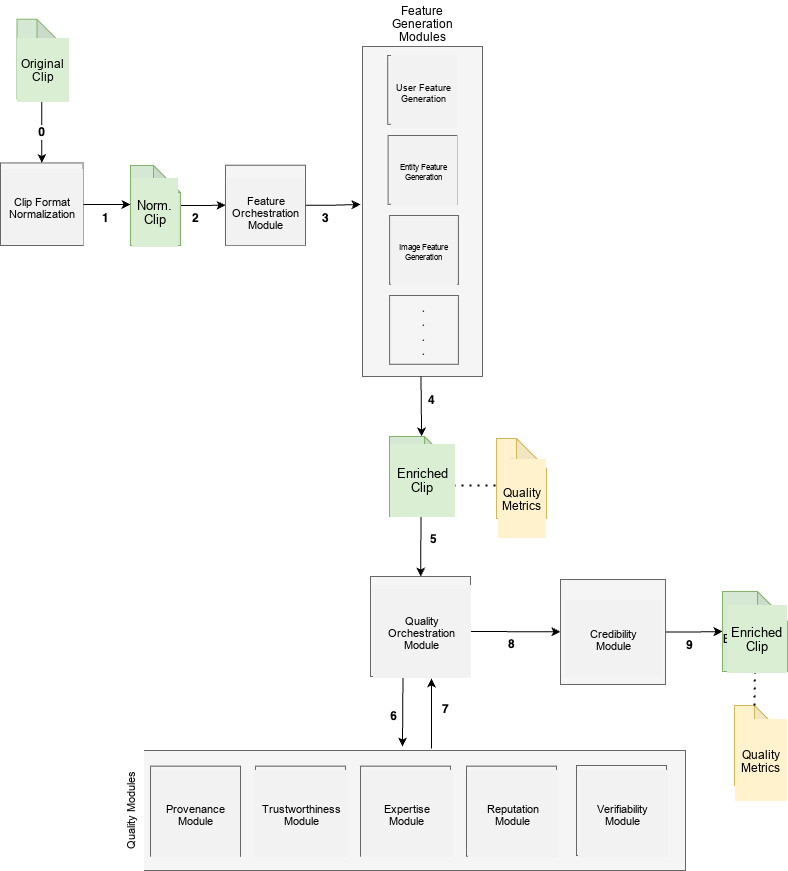
\includegraphics[width=.64\textwidth,keepaspectratio]{figures/processing-flow-en}
  \caption{Modular processing flow for credibility assessment~\cite{GarciaParra2024Thesis}.}
  \Description{Processing flow from original clip to normalized clip, feature generation, quality modules, and enriched clip.}
  \label{fig:processing-flow}
\end{figure*}

\autoref{fig:processing-flow} summarizes the logical workflow. The normalized clip
is the contract between platform-specific ingestion and quality computation. This
contract is important because social platforms expose different fields, policies,
and APIs. A normalized clip contains the content, platform URI, author metadata,
links, mentions, reactions, comments, feature outputs, and quality metrics needed
by downstream modules.

The feature-generation stage is intentionally separated from the quality-metric
stage. A feature module may extract a medical profession from a user profile,
detect whether an institution is mentioned, compute audience size, or identify
external links. A quality module then maps those features to a value in $[0,1]$,
using a formula, a rule, or a model. This separation lets a new feature extractor
be added without changing the semantics of the quality model.

The provenance module distinguishes explicit and implicit interactions. Explicit
interactions are represented by platform mechanisms such as retweets, replies,
quotes, or shares. Implicit interactions occur when users copy, paraphrase, or
repost content without preserving a direct platform link. These cases are common
in cross-sharing, where content moves between platforms and may lose its original
metadata.

\begin{figure*}[t]
  \centering
  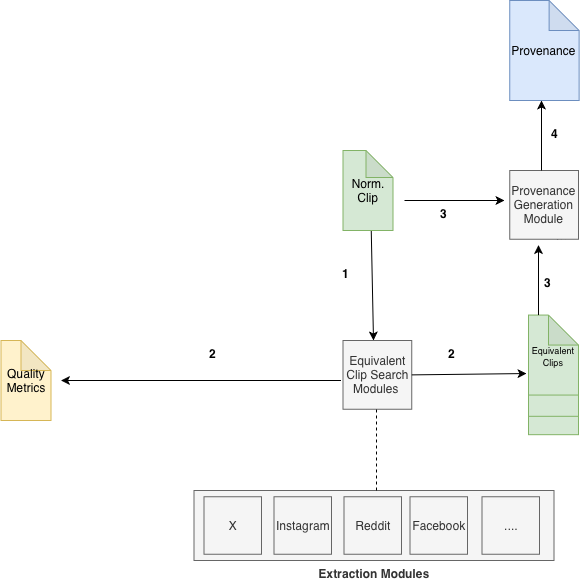
\includegraphics[width=.62\textwidth,keepaspectratio]{figures/provenance-framework-en}
  \caption{Framework for searching equivalent clips and generating provenance~\cite{GarciaParra2024Thesis}.}
  \Description{Provenance generation workflow with normalized clips, equivalent-clip search modules, extracted clips, metrics, and provenance output.}
  \label{fig:provenance-framework}
\end{figure*}

To address implicit interactions, the flow uses clip equivalence. For text clips,
we instantiate equivalence with TF-IDF cosine similarity~\cite{Yuntao2005}. Given
two clips $c_1$ and $c_2$, their textual similarity is:
\begin{equation}
  Sim(c_1,c_2) = \frac{c_1 \cdot c_2}{\|c_1\|\|c_2\|}.
\end{equation}
Equivalent clips are then mapped to a provenance representation inspired by
PROV-SAID. We adapt PROV-SAID by replacing messages with clips, adding an
attribute for the social network, modeling cross-platform derivations, and
attaching quality metrics such as trustworthiness, verifiability, expertise, and
reputation to provenance entities.

\autoref{fig:provenance-framework} depicts this sub-flow. The equivalent-clip
search module can use exact matching, approximate matching, semantic search, query
expansion, multilingual search, or contextual search with hashtags, URLs, dates,
and user mentions. In the current proof of concept, we restrict the equivalence
metric to text clips, but the model allows future multimodal equivalence metrics
for images and videos.

\subsection{Trustworthiness Path Stability}

The main provenance-derived metric is \emph{Trustworthiness Path Stability}. It
measures whether trustworthiness remains stable as a clip propagates. Let
$T_i$ be the trustworthiness value of the $i$-th clip in a provenance path of
length $n$. We define:
\begin{equation}
  TPS = 1 - \frac{\sum_{i=1}^{n-1}|T_{i+1}-T_i|}{n-1}.
\end{equation}
Since each $T_i$ is normalized in $[0,1]$, each consecutive difference is also in
$[0,1]$. Therefore, for paths with $n \geq 2$, $TPS$ ranges from 0 to 1. Values
close to 1 indicate stable trustworthiness across the path. Lower values indicate
fluctuations, possibly caused by content modifications, loss of source quality, or
propagation through less trustworthy actors. When a clip has no provenance path
or the path contains a single clip ($n=1$), $TPS$ is not computed because there is
no consecutive transition to evaluate.

For example, consider a path with trustworthiness values 0.90, 0.85, 0.88, and
0.86. The total variation between consecutive nodes is
$0.05+0.03+0.02=0.10$, and therefore $TPS=1-0.10/3=0.9667$. The resulting value
indicates that credibility was not materially degraded along the path. This is
useful for cross-platform sharing because the same content can preserve its claim
while being copied into a different social context.

\section{Proof of Concept}

We implemented a proof of concept for health-related social media clips about
statins and cholesterol. This domain was selected because misinformation about
statins can influence treatment adherence and public-health decisions. The
implementation was deployed on Google Cloud Platform using Pub/Sub for ingestion,
Cloud Storage for persistence, Cloud Functions for feature and quality modules,
and Cloud Composer for orchestration.

The experiment started from 97 clips collected from multiple social media
platforms using keywords related to statins and cholesterol. Eleven clips were
preselected to cover different platforms and credibility levels. A medical-domain
expert classified the selected clips into credibility levels and provided scores.

For the experiment, trustworthiness was computed from three metrics: access to
source data, certification, and confidence. The domain expert assigned weights of
0.4, 0.4, and 0.2, respectively. Credibility combined Trustworthiness Path
Stability and trustworthiness with weights of 0.6 and 0.4 when provenance was
available. When no provenance was available, the model relied only on
trustworthiness.

In this proof of concept, the feature modules focused on medical profile evidence. They
extracted medical profession, medical education, medical verifiability, and
medical influence from public profile information and available textual evidence.
The quality modules then computed certification, access to source data, confidence,
trustworthiness, Trustworthiness Path Stability, and final credibility. Thresholds
were conservative: values from 0.00 to 0.50 were considered low credibility,
0.51 to 0.75 medium, and 0.76 to 1.00 high.

\begin{table}[t]
  \caption{Comparison between expert judgments and model output~\cite{GarciaParra2024Thesis}.}
  \label{tab:results}
  \begin{tabular}{ccccc}
    \toprule
    Clip & Expert & Score & Model & Cred.\\
    \midrule
    1 & Medium & 0.60 & High & 0.80\\
    2 & Medium & 0.70 & Medium & 0.68\\
    3 & Medium & 0.60 & Medium & 0.68\\
    4 & Medium & 0.70 & Medium & 0.64\\
    5 & Medium & 0.60 & High & 0.78\\
    6 & Low & 0.00 & Low & 0.09\\
    7 & Low & 0.00 & Low & 0.18\\
    8 & Low & 0.00 & Low & 0.11\\
    9 & Low & 0.10 & Low & 0.09\\
    10 & Low & 0.00 & Low & 0.08\\
    11 & Low & 0.00 & Low & 0.36\\
    \bottomrule
  \end{tabular}
\end{table}

The model agreed with the expert level in nine of the eleven clips
(\autoref{tab:results}). The two differences corresponded to clips for which
provenance increased the credibility score: both had stable paths and were shared
by users with relatively high trustworthiness. The expert did not have access to
all profiles involved in the cross-platform propagation path, which explains why
the expert score was closer to trustworthiness alone than to the final
provenance-aware score.

Three qualitative examples illustrate this effect. Clip 1 was associated with a
cardiology profile with high certification and audience confidence, but limited
explicit access to source data. Its trustworthiness score was therefore medium
($0.62$). However, the clip was propagated through a stable path with high
Trustworthiness Path Stability ($0.92$), which raised its final credibility to
$0.80$. Clip 5 followed a similar pattern: stronger source and certification
signals yielded medium trustworthiness ($0.69$), and a stable provenance path
($0.83$) raised the final score to $0.78$. In both cases, the qualitative
explanation is not that the original clip was automatically high credibility, but
that provenance added evidence unavailable in the expert's isolated view.
Conversely, Clip 7 came from a self-described naturopath profile, with weak
certification and limited verifiable source evidence; it remained low credibility
($0.18$) despite having some audience-related signals.

The preliminary implementation had an average execution time of 5220 ms per clip.
The sample is too small for claims about scalability or predictive accuracy. The
value of the experiment is instead to show that a data-quality model can produce
interpretable credibility metrics and expose where provenance changes the
assessment.

The detailed metrics also show why the model produced these results. Clips
published by accounts with explicit medical credentials and verifiable institutional
references obtained higher certification and access-to-source-data values. Clips
from self-proclaimed or pseudoscientific profiles obtained low expertise values
even when they had audience signals. Confidence had a smaller weight to avoid
overvaluing popularity in a sensitive medical domain.

\section{Discussion, Future Work, and Conclusion}

The proposed model shifts credibility assessment from a monolithic prediction
task to a data-quality workflow. The first advantage is explicitness: users can
inspect whether a score came from source verifiability, author expertise,
reputation, or provenance stability. The second is adaptability. Medical
credibility can use certification and access to source data, while other domains
may define different features and thresholds.

There are also limitations. The proof of concept uses a small set of clips and a
single domain expert. The clip-equivalence strategy is limited to text and does not
yet cover images or video. The provenance reconstruction depends on platform APIs,
search engines, and available public metadata. Finally, the model assumes that
domain experts can define meaningful weights; future work should compare manual,
rule-based, and machine-learned weight calibration.

\noindent\textbf{Future work.} Future work should expand the evaluation to larger datasets, additional social
media platforms, and multiple domain experts in order to measure inter-rater
agreement and domain transferability. A second line of work is multimodal clip
equivalence, including images, video, screenshots, and partial paraphrases, since
misleading content is often propagated through format changes rather than exact
textual reuse. The current proof of concept uses TF-IDF as a transparent baseline
for text-only equivalence. Future versions should evaluate whether small language
models (SLMs) can replace or complement it for semantic clip equivalence,
especially when content is paraphrased, translated, rendered as an image, or
moved across platforms. SLMs are also relevant for image-based clip processing,
such as screenshots or rendered posts, because access to social media APIs is
increasingly restricted and heterogeneous across platforms. These SLMs should run
at the edge, without sending clips to the cloud, to preserve privacy. The
credibility quality model should be integrated into the SLM pipeline so that
extracted visual and textual evidence is mapped directly to quality dimensions
and metrics. The provenance component should also be extended with explicit
quality metadata for completeness, confidence, uncertainty, and missing links.
Finally, the model requires further work on weight calibration and user-facing
visualizations that explain how each quality dimension contributes to the final
credibility score.

\noindent\textbf{Conclusion.} This paper presented a provenance-aware data-quality model for measuring
credibility in social media platforms. By combining trustworthiness, provenance,
clip equivalence, and Trustworthiness Path Stability, the model provides an
interpretable way to evaluate social media content across platforms and domains.
The proof of concept in the statins domain suggests that provenance can materially
change credibility assessment and should be treated as a first-class quality signal.
A more detailed account of the model and its design rationale is available in
the master's thesis~\cite{GarciaParra2024Thesis}; the code repository is available at
\url{https://github.com/dsgarcia/clips-credibility}.

\begin{acks}
This work was partially funded by Comisión Sectorial de Investigación Científica (CSIC), Universidad de la República, Uruguay.
\end{acks}

\bibliographystyle{ACM-Reference-Format}
\bibliography{references}

\end{document}
\endinput
